\documentclass[12pt,a4paper]{article}

% ------------------------------------------------
% Packages
% ------------------------------------------------
\usepackage[utf8]{inputenc}
\usepackage[T1]{fontenc}
\usepackage[french]{babel}
\usepackage{graphicx}
\usepackage{geometry}
\usepackage{xcolor}
\usepackage{lmodern}
\usepackage{setspace}
\usepackage{graphicx}
\usepackage{float}
\usepackage{blindtext}
\usepackage{hyperref}
\usepackage{longtable}
\usepackage{booktabs}

\geometry{
    top=2.5cm,
    bottom=2.5cm,
    left=2.5cm,
    right=2.5cm
}

\definecolor{ensaiBlue}{RGB}{47,91,140}

\begin{document}

% ==================================================
% PAGE DE GARDE
% ==================================================

\begin{titlepage}

\begin{center}

% ------------------------------------------------
% Logo ENSAI
% ------------------------------------------------

\IfFileExists{logo_ensai2.jpg}{
    
\includegraphics[width=0.32\textwidth]{logo_ensai2.jpg}
}{
    {\Large \textbf{ENSAI}}
}

\vspace{1.2cm}

% ------------------------------------------------
% École / Formation
% ------------------------------------------------

\vspace{0.4cm}

{\large
Deuxième année -- Projet informatique
}

\vfill

% ------------------------------------------------
% Projet
% ------------------------------------------------

{\color{ensaiBlue}
\rule{\textwidth}{1.2pt}
}

\vspace{0.7cm}

{\Huge \bfseries ANONYMIA}

\vspace{0.3cm}

{\Large \textbf{Groupe 21}}

\vspace{0.4cm}

{\Large
Application d'anonymisation\\
de documents administratifs
}

\vspace{0.8cm}

{\color{ensaiBlue}
\rule{\textwidth}{1.2pt}
}

\vspace{1.4cm}

% ------------------------------------------------
% Type de document
% ------------------------------------------------

{\LARGE \bfseries Document d'analyse}

\vspace{0.4cm}

{\large
Analyse du besoin et conception fonctionnelle
}

\vfill

% ------------------------------------------------
% Membres du groupe
% ------------------------------------------------

\begin{minipage}{0.75\textwidth}

\centering

{\large \textbf{Équipe projet}}

\vspace{0.5cm}

\begin{tabular}{c}
ALVES Ryan \\[0.2cm]
HAUET Noah \\[0.2cm]
KUATE Cabrel\\[0.2cm]
LE BESNERAIS Tom \\[0.2cm]
LE DOARÉ Tanguy
\end{tabular}

\vspace{1cm}

{\large
\textbf{Tuteur :} LAGALLE Maxence
}

\end{minipage}

\vfill

% ------------------------------------------------
% Date
% ------------------------------------------------

{\large
Année universitaire 2026--2027
}

\vspace{0.3cm}


\end{center}

\end{titlepage}

% ==================================================
% SUITE DU DOCUMENT
% ==================================================

\tableofcontents
\newpage

\section{Expression du besoin}

Les documents administratifs (courriers, factures, contrats…) contiennent très souvent des données personnelles, comme des noms, des adresses, voire même des coordonnées bancaires, qui peuvent être très sensibles et doivent donc éviter tout risque de fuite ; or cela peut arriver lorsque l’on partage ces données, par exemple pour les archiver. Selon le règlement général sur la protection des données (RGPD), ces informations doivent donc être protégées le mieux possible ; on peut pour cela utiliser par exemple la technique du caviardage, mais c’est une tâche qui peut être très longue et sujette à l’erreur.

C’est dans ce contexte que s’inscrit notre projet Anonymia : notre but est de créer une application qui soit capable de détecter automatiquement les données confidentielles qui sont présentes dans un document fourni, puis de les caviarder. De plus, il faut que le texte fourni soit encore lisible et qu’il ait du sens.
\newline

Pour détecter les éléments à caviarder, nous avons utilisé deux approches différentes qui se complètent : une méthode “régulière” pour les types de données avec un format toujours identique, comme l’IBAN ou le numéro de sécurité sociale, et un grand modèle de langage (LLM) pour les données dont le format peut varier, comme des noms de personnes ou des lieux. Cette application doit de plus pouvoir continuer de fonctionner même si le modèle de langage est indisponible, et doit pouvoir se défendre contre les injections de prompt qui seraient dans le contenu des documents analysés.
\newline

Ce document présente notre démarche d’analyse et de conception de cette application : l’architecture logicielle que nous avons adoptée, la modélisation du système à l’aide de plusieurs ammeammes UML (diagramme de cas d’utilisation / de classes / séquences) et [j’ai pas la suite]



\section{Analyse fonctionnelle}
\subsection{Description des fonctionnalités}

Notre application Anonymia offrira un panel de fonctionnalités pour le traitement des documents administratifs, dont les principales sont :

\begin{itemize}
\item un système d'authentification et de gestion des comptes utilisant l'application : l'administrateur a la possibilité de gérer les profils Superviseur et Utilisateur (les créer, supprimer/désactiver ou modifier les rôles), obtenir des tokens pour les requêtes HTTP ;
\item la détection des PII et de leur emplacement par deux moteurs de détection distincts qui fonctionnent en parallèle : un déterministe (Regex) et un probabiliste/contextuel (LLM) ;
\item l'anonymisation du document : modification du contenu du texte selon une stratégie différenciée pour chaque type de PII (au choix de l'utilisateur), voir l'illustration ci-dessous :
\item le suivi des traitements : des métadonnéees qui décrivent le traitement du document et les types de PII détectés sont mis à disposition des superviseurs et administrateurs ;
\item sécurisation en couches du détecteur LLM : pour prémunir le système contre les attaques par injection de prompt (l'une des plus grandes menaces contre un LLM), les fuites de contexte ou encore la génération de formats invalides, une protection à trois niveaux a été mise en place (prompt système strict afin de signifier au LLM qu'il ne doit pas suivre d'instruction dans le corps du texte, un pré-filtrage ainsi qu'une vérification de la sortie via Pydantic).
\end{itemize}

Disclaimer :
Aucun système automatisé d'analyse du langage naturel (LLM) ni aucune suite d'expressions régulières ne peut garantir un rappel de 100 \% sur des documents administratifs non structurés. En raison des variations de syntaxe, des erreurs de typographie et des ambiguïtés contextuelles, des PII peuvent ne pas être détectées (faux négatifs). L'outil constitue une aide à la décision et un gain de temps en automatisant une tâche souvent fastidieuse : une relecture humaine systématique reste obligatoire avant toute publication ou diffusion de documents caviardés.

\subsection{Description des couches de l'application}

L'application que nous allons proposer est d'importance suffisante pour qu'il soit préferable de la segementer en différentes couches, afin de permettre une meilleure organisation. Pour cela, nous pouvons essayer de suivre le principe de "séparation des responsabilités" (separation of concerns ou SoC en anglais). Ce principe préconise d'isoler les parties du code ayant une fonction précise relativement à la problématique générale. Il favorise notamment le travail en équipe, le déboggage et la lisibilité du code. L'application finale sera ainsi dotée de ces trois couches principales:

\subsubsection{La couche de présentation (Presentation layer)}
Cette couche communique directement avec le client. Elle correspond au front-end de notre application, écrit en Python et utilisant le framework \href{https://streamlit.io/}{Streamlit}. Cette couche ne sera pas détaillée dans la suite de ce rapport, où l'on portera plus d'attention aux deux autres couches.

\subsubsection{La couche de traitement (Business layer)}
C'est cette couche qui englobe la partie logique de l'application. Elle communique avec l'application sous forme d'une API de type \href{https://fr.wikipedia.org/wiki/Representational_state_transfer}{REST} de préférence. L'outil utilisé pour cela est \href{https://fastapi.tiangolo.com/}{FastAPI}. Plus générallement, elle a les missions suivantes:
\begin{itemize}
\item Gérer les utilisateurs (création de compte, authentification, gestion des rôles, etc.)
\item Recevoir les documents à caviarder
\item Caviarder les documents selon les paramètrages de l'utilisateur
\item Communiquer avec la base de données.
\end{itemize}

La complexité de cette tâche entraîne une nouvelle segmentation cette couche en sous-couches, chacune ayant leur responsabilités propres:
\begin{enumerate}
\label{sec:controle}
\item La couche de contrôle, qui reçoit les requêtes HTTP du client et communique les réponses en se servant la couche de service. Pour faciliter le traitement de ces requêtes, FastAPI propose des \textit{modèles}, qui sont des classes de données utiles pour structurer les requêtes entrantes et sortantes de l'API.
\item La couche de service, qui propose des services qui traitent les appels provenant principalement de la couche de contrôle. Il est prévu que cette couche propose deux services: un service qui traite les appels relatifs aux utilisateurs (création de compte, liste des comptes, etc.) et un autre qui traite les appels relatifs aux documents (création et caviardage d'un document, liste des documents caviardés).
\item La couche d'accès aux données, qui constitue une interface communiquant avec la base de données. La base de données correspond à la couche de persistance. Pour réaliser des requêtes sur cette base, on utilise le module \href{https://www.psycopg.org/}{psycopg2}. 
\item La couche "Business", qui modélise les objets qui seront utilisés par le couche de traitement dans son ensemble, c'est à dire qui sont utilisés par la couche de service et d'accès aux données pour modéliser les joueurs et les documents, et ces objets peuvent être communiqués d'une couche à une autre.
\end{enumerate}

\subsubsection{La couche de persistance (Persistence layer)}
La couche de persistance constitue la base de donnée à laquelle fait appel l'application Python. Nous utilisons pour cela le système de gestion de base de données PostgreSQL, parce qu'il est réputé robuste et qu'il est disponible sur Onyxia. 

\subsection{Choix}

Cette section présente les principaux choix retenus dans notre analyse. 
Ils concernent d'une part la typologie des données personnelles détectées 
par Anonymia et, d'autre part, les règles permettant de trancher les cas 
dont le caractère identifiant dépend davantage du contexte.

\subsubsection{Liste des PII}

Les PII retenues sont classées selon trois cercles correspondant à un niveau
croissant de difficulté de détection. Plus on s'éloigne du premier cercle,
plus la décision de détection relève d'un choix de conception à documenter,
et non d'une évidence technique.

\medskip
\noindent\textbf{Cercle 1 --- Identification directe et non ambiguë}

\smallskip

Ces types identifient une personne à eux seuls, sans nécessiter de mise en
contexte ni de recoupement. Aucune règle de décision particulière n'est
requise : la présence de la donnée suffit.

\renewcommand{\arraystretch}{1.3}
\begin{longtable}{
    p{3.2cm}
    @{\hspace{0.4cm}}
    p{1.8cm}
    @{\hspace{0.4cm}}
    p{8.5cm}
}
\toprule
\textbf{Type} & \textbf{Détecteur} & \textbf{Justification} \\
\midrule
\endhead

NIR (Numéro d’Inscription au Répertoire)
& Regex
& Structure fixe avec clé de contrôle calculée à partir des autres chiffres ;
identifiant unique d'une personne à lui seul, sans besoin d'aucune autre
information. \\

IBAN (International Bank Account Number)
& Regex
& Format international normalisé, vérifiable par clé de contrôle
(modulo 97) ; désigne un compte bancaire rattaché à une personne physique. \\

Mail
& Regex
& Structure fixe (partie locale, arobase, domaine) ; très souvent nominative
ou directement rattachable à un individu. \\

Numéro de téléphone
& Regex
& Format national relativement structuré (nombre de chiffres, préfixe) ;
un numéro, surtout mobile, est généralement propre à un seul individu. \\

Numéro CNI (Carte nationale d'identité)
& Regex
& Structure fixe ; il constitue un identifiant administratif unique de son
détenteur. \\

PAN (Primary Account Number)
& Regex
& Format structuré selon le réseau émetteur et vérifiable par l'algorithme
de Luhn ; donnée financière directement rattachée à son porteur. \\

Nom de personne
& LLM
& Aucune structure syntaxique propre ; la compréhension du contexte permet
d'identifier un nom propre désignant une personne. Il s'agit d'un des types
les plus difficiles à détecter. \\

Adresse postale avec code postal
& LLM
& Forme libre (numéro, rue, ville) qu'aucun motif unique ne peut couvrir dans
toute sa variété ; elle permet de localiser précisément le domicile d'une
personne. \\

\bottomrule
\end{longtable}


\medskip
\noindent\textbf{Cercle 2 --- Identification indirecte ou dépendante du contexte}

\smallskip

Ces types nécessitent un recoupement avec d'autres informations ou une règle
de décision permettant de déterminer leur caractère identifiant.

\begin{longtable}{
    p{3.2cm}
    @{\hspace{0.4cm}}
    p{1.8cm}
    @{\hspace{0.4cm}}
    p{8.5cm}
}
\toprule
\textbf{Type} & \textbf{Détecteur} & \textbf{Justification et règle de décision} \\
\midrule
\endhead

Plaque d'immatriculation
& Regex
& Format réglementé et fixe (par exemple AA-123-AA) ; identifie un véhicule
et peut indirectement permettre de remonter à son propriétaire. \\

Adresse IP
& Regex
& Format structuré (IPv4 ou IPv6) ; via le fournisseur d'accès, elle peut
permettre de remonter jusqu'à un foyer ou un individu. \\

SIREN (Système d’Identification du Répertoire des Entreprises)
& Regex
& Longueur et structure fixes ; identifie en principe une entreprise.
\textbf{Règle :} il n'est retenu comme donnée personnelle que lorsqu'il
concerne une entreprise individuelle ou une activité permettant d'identifier
directement une personne physique. \\

Référence cadastrale
& Regex
& Codification structurée permettant d'identifier une parcelle ; le
recoupement avec des registres peut permettre de retrouver son propriétaire. \\

Données GPS
& Regex
& Coordonnées numériques structurées ; une position suffisamment précise
peut révéler un domicile ou des habitudes de déplacement. \\

Date de naissance
& LLM
& Une date seule ne permet pas de déterminer la nature de l'événement.
\textbf{Règle :} elle est retenue comme date de naissance uniquement lorsque
le contexte l'associe explicitement à une naissance. \\

Lieu
& LLM
& Aucune structure permettant à elle seule de déterminer son caractère
identifiant. La décision dépend du contexte et notamment du niveau de
précision géographique. \\

Organisme
& LLM
& Le caractère identifiant dépend de la taille de la structure. Une
institution nationale ne permet généralement pas d'identifier une personne,
contrairement à une structure très restreinte. \\

\bottomrule
\end{longtable}


\medskip
\noindent\textbf{Cercle 3 --- Jugement fortement contextuel et catégories sensibles}

\smallskip

Ces types nécessitent une interprétation fine du texte ou un cumul
d'informations. Leur détection repose donc principalement sur le contexte.

\begin{longtable}{
    p{3.2cm}
    @{\hspace{0.4cm}}
    p{1.8cm}
    @{\hspace{0.4cm}}
    p{8.5cm}
}
\toprule
\textbf{Type} & \textbf{Détecteur} & \textbf{Justification} \\
\midrule
\endhead

Fonctions révélatrices
& LLM
& Un intitulé de fonction seul est peu identifiant, mais combiné à une
organisation ou à un lieu précis, il peut permettre d'identifier une personne. \\

Liens familiaux
& LLM
& Une mention telle que « son fils » ou « sa femme » ne désigne pas directement
une personne, mais peut devenir identifiante lorsqu'elle est combinée à
d'autres éléments du texte. \\

Éléments de vie privée (cumul)
& LLM
& Chaque détail pris isolément peut sembler anodin ; leur accumulation peut
permettre de réidentifier une personne par recoupement. \\

Situation judiciaire
& LLM
& Information particulièrement sensible dont la détection dépend entièrement
du contexte et de la formulation employée. \\

Revenus d'une personne physique
& LLM
& Donnée financière personnelle à distinguer du chiffre d'affaires d'une
entreprise, qui concerne une structure et non directement un individu. \\

Suivi médical
& LLM
& Donnée nécessitant une compréhension du contexte médical, sans structure
syntaxique fixe permettant une détection par expression régulière. \\

Ethnie
& LLM
& Donnée sensible dont l'identification repose principalement sur
l'interprétation du texte. \\

Sexe et accords grammaticaux
& LLM
& Information pouvant être utile pour maintenir la cohérence grammaticale lors
d'une pseudonymisation ; elle n'est pas nécessairement occultée de manière
systématique. \\

\bottomrule
\end{longtable}


\subsubsection{Règles}

Au-delà de la typologie précédente, certaines situations nécessitent des règles
explicites afin de déterminer si une information doit être considérée comme
suffisamment identifiante pour être détectée et traitée par Anonymia.

\medskip
\noindent\textbf{Règles d'inclusion et seuils}

\smallskip

\textbf{Commune de moins de 10\,000 habitants $\Rightarrow$ révélatrice.}
Plus une commune compte peu d'habitants, plus le nombre de personnes
correspondant à un profil donné y est restreint. Lorsqu'elle est combinée à
d'autres informations telles que l'âge, la fonction ou la situation familiale,
une localisation précise peut donc faciliter la réidentification. Un seuil
permet d'appliquer cette règle de manière homogène.

\medskip

\textbf{Tranches d'âge plutôt qu'âge exact.}
Un âge exact peut devenir fortement identifiant lorsqu'il est combiné à d'autres
informations. Lorsque l'âge doit être conservé pour préserver le sens du
document, l'utilisation d'une tranche d'âge permet de diminuer la précision de
l'information tout en conservant son intérêt.

\medskip

\textbf{Retrait du jour et du mois pour certaines dates liées à un événement.}
Une date complète associée à un événement particulier peut faciliter un
recoupement avec des sources externes. Lorsque la précision complète n'est pas
nécessaire à la compréhension du document, seule l'année peut être conservée.

\medskip
\noindent\textbf{Règles d'exclusion}

\smallskip

\textbf{Zones géographiques larges.}
Une zone géographique suffisamment large regroupe un grand nombre d'individus et
ne permet généralement pas, à elle seule, d'identifier une personne. Son
occultation pourrait alors appauvrir inutilement le document.

\medskip

\textbf{Personnalités publiques.}
Lorsqu'une personne est mentionnée dans le cadre de fonctions publiques ou
d'informations déjà largement accessibles, son traitement peut différer de
celui d'une personne privée. Ce choix doit néanmoins être apprécié en fonction
du contexte du document.

\subsection{Sécurité}

La sécurité constitue un enjeu central d'Anonymia, puisque l'application est amenée à manipuler des documents contenant potentiellement des données personnelles sensibles. Elle concerne à la fois la protection des compte utilisateurs, la conservation des données traitées et la sécurisation de
l'utilisation du modèle de langage.

Concernant l'authentification, les mots de passe des utilisateurs ne sont jamais stockés en clair dans la base de données. Seule une version hachée est conservée, de sorte qu'une compromission de la base ne permette pas d'accéder directement aux mots de passe. Les droits d'accès sont également limités selon trois rôles :
utilisateur, superviseur et administrateur. Cette séparation permet de restreindre l'accès aux fonctionnalités sensibles, notamment la gestion des comptes et la consultation de l'historique des traitements.

Une attention particulière est également portée aux documents soumis à l'application. Le contenu brut d'un document n'a pas vocation à être enregistré de manière permanente. La journalisation conserve uniquement les métadonnées
nécessaires au suivi du traitement, telles que l'utilisateur, la date, les détecteurs utilisés ou le nombre de PII détectées. Une empreinte cryptographique du document peut également être calculée afin de pouvoir identifier qu'un document a déjà été traité sans avoir à conserver son contenu.

L'utilisation d'un LLM introduit par ailleurs un risque spécifique d'injection de prompt. Un document soumis par l'utilisateur peut contenir des instructions malveillantes afin de pousser le modèle à ne pas détecter certaines PII. Si une telle attaque réussissait, des données personnelles pourraient rester présentes dans le document final. Pour limiter ce risque, Anonymia repose sur une défense en profondeur en trois
étapes. Tout d'abord, un prompt système strict rappelle au modèle que le document constitue uniquement une donnée à analyser et que les instructions qu'il contient ne doivent pas être exécutées. Ensuite, un \texttt{InjectionFilter} recherche
avant l'appel au LLM des motifs susceptibles de correspondre à une tentative d'injection. Enfin, la sortie du modèle est contrôlée par un \texttt{OutputVerifier}, qui vérifie le respect du format attendu, la validité des types de PII retournés ainsi que la présence réelle dans le document des
éléments signalés par le modèle.

Aucune de ces protections n'étant suffisante isolément, leur combinaison permet de réduire le risque d'une sortie incorrecte ou manipulée. Le détecteur Regex constitue également un niveau de sécurité supplémentaire, puisqu'il ne dépend pas des instructions présentes dans le document. En cas d'échec ou
d'indisponibilité du LLM, l'application peut ainsi continuer à fonctionner en mode dégradé à partir des résultats issus des expressions régulières.

\subsection{Technologies}

\textbf{Backend et API}


Anonymia repose sur \textbf{FastAPI}, un framework web Python, qui permet de lancer en parallèle les deux détecteurs de PII sans qu’ils se bloquent, notamment en fonction du temps utilisé, car le modèle de langage est plus lent que le détecteur par expressions régulières.
\newline

\textbf{Interface utilisateur}


L'interface est développée avec \textbf{Streamlit}, une bibliothèque Python qui permet de construire une application web interactive sans HTML, CSS ou JavaScript.
\newline

\textbf{Gestion de l'environnement Python}


Nous utilisons \textbf{uv} pour gérer les dépendances et l'environnement virtuel du projet, car ill garantit que l'environnement soit exactement le même pour tous nos ordinateurs : lorsqu'un membre clone le dépôt, la commande de synchronisation reconstitue à l'identique l'ensemble des dépendances, ce qui élimine les écarts de configuration.
\newline

\textbf{Base de données}


Pour stocker les données persistantes du projet, comme les comptes des utilisateurs (avec les mots de passe hashés), ou les documents traités et leur métadonnées, nous utilisons \textbf{PostgreSQL}, disponible via le Datalab.
\newline

\textbf{Intégration du modèle de langage}


Pour la détection des PII à format libre, nous avons fait appel à un grand modèle de langage (LLM), qui est exposé par l'\textbf{API LLM du Datalab SSP Cloud} :  en effet, les documents traités contenant des données personnelles, il est interdit de les transmettre à une API commerciale externe, car cela correspondrait à une fuite.

L'accès au LLM s'effectue au moyen d'une clé API personnelle, stockée dans un fichier .env qui est exclu du versionnement. L'accès au LLM s'effectue au moyen d'une clé API personnelle, stockée dans un fichier .env qui est exclu du versionnement. L'API du SSP Cloud est compatible avec le standard OpenAI, ce qui permet d'exécuter des modèles localement grâce à Ollama, car ils utilisent tous les deux la bibliothèque \textbf{openai} de Python.




\section{Diagrammes}
\subsection{Diagramme de cas d'utilisation}

Notre application propose des fonctionnalités en réponse directe aux besoins formulés précédemment. Ainsi, l'administrateur aura la possibilité de créer un compte, le désactiver, le supprimer, ou même en modifier le rôle. Une fois connecté à son compte, le superviseur peut consulter les métadonnées d'un document traité en filtrant par utilisateur ou par période. Enfin, l'utilisateur pourra réaliser le métier de caviardage : lorsqu'il importe un document, celui-ci pourra être analysé avec une détection des données personnelles et une stratégie d'anonymisation au choix de l'utilisateur, tout en assurant une journalisation du traitement.
Nous avons fait le choix d'une logique d'emboîtement (héritage) des profils d'utilisation : un administrateur possède les fonctions d'un superviseur qui lui-même peut réaliser les actions d'un utilisateur.

\subsection{Diagrammes d'activité}

\begin{figure}[H]
    \centering
    \includegraphics[width=0.65\textwidth]{Diagramme d'activité.png}
    \caption{Diagramme d'activité du traitement d'un document}
    \label{fig:activité}
\end{figure}

Ce diagramme modélise l'ensemble du processus qu'un utilisateur traverse, de l'authentification à la récupération du document caviardé. Après vérification de ses identifiants (et éventuellement une modification de ceux-ci), l'utilisateur dépose le document à analyser. Le système lance alors en parallèle la détection par expressions régulières (pour les formats fixes) et par modèle de langage (pour les formats libres), vérifie la validité de la sortie LLM, puis fusionne les résultats. L'utilisateur choisit ensuite la stratégie d'anonymisation : soit masquage, soit pseudonymisation cohérente. Le système applique alors le traitement correspondant, puis la liste des données personnelles détectées est affichée à l'écran, et l'utilisateur récupère enfin le document caviardé.

\subsection{Diagramme de séquence}

\begin{figure}[H]
    \centering
    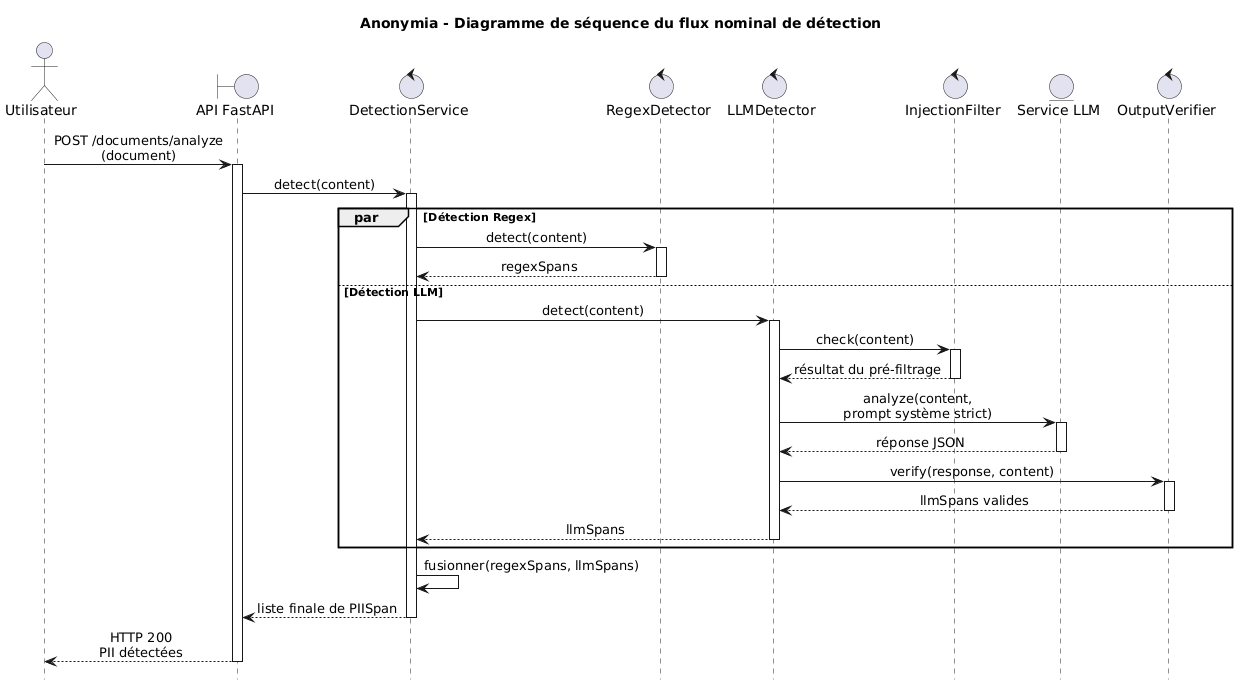
\includegraphics[width=\textwidth]{diagramme_sequence.png}
    \caption{Diagramme de séquence du flux nominal de détection des PII}
    \label{fig:sequence-detection}
\end{figure}

Le diagramme de séquence présenté en figure~\ref{fig:sequence-detection}
décrit le flux nominal de détection des données personnelles. Lorsqu'un utilisateur soumet un document, la requête est reçue
par l'API FastAPI puis transmise au \texttt{DocService}. Celui-ci fait appel à l'\texttt{AnalyserFactory} afin d'obtenir un analyseur adapté aux paramètres du traitement. L'objet retourné respecte l'interface \texttt{Analyser} et est ensuite utilisé par le \texttt{DocService} pour lancer l'analyse du contenu.

L'analyseur déclenche en parallèle les deux mécanismes de détection. Le \texttt{RegexDecorator} recherche les PII dont la forme peut être caractérisée par des motifs prédéfinis, tandis que le \texttt{LLMDecorator} prend en charge les informations nécessitant davantage de contexte. Avant l'appel au modèle,
le document passe par un \texttt{InjectionFilter} chargé de repérer d'éventuelles tentatives d'injection de prompt. La réponse du LLM est ensuite contrôlée par un \texttt{OutputVerifier}, qui vérifie notamment la conformité du format retourné, la validité des types de PII ainsi que la présence effective dans le document des textes identifiés par le modèle. Il permet également de retrouver de manière déterministe les positions correspondant aux PII détectées.

Lorsque les deux traitements sont terminés, leurs résultats, représentés sous forme de \texttt{Positions}, sont fusionnés afin d'obtenir l'ensemble final des PII détectées. Ce résultat est ensuite transmis au \texttt{DocService}, puis à l'API FastAPI qui le retourne à l'utilisateur.

En cas d'indisponibilité ou d'échec du traitement par le LLM, l'application fonctionne en mode dégradé : l'analyse peut se poursuivre à partir des résultats obtenus par le \texttt{RegexDecorator}. L'échec du LLM ne provoque donc pas
l'arrêt complet du traitement.

\subsection{Diagramme des classes}

\begin{figure}[H]
    \centering
    \includegraphics[width=\textwidth]{diagramme_classes2.png}
    \caption{Diagramme des classes - Types et modèles}
    \label{fig:classes1}
\end{figure}

Tout d'abord, nous devons décrire les types personnalisés utilisés dans le projet. Afin de favoriser la clarité de la lecture, les liens entre les types représentés ici et les classes du deuxièm( e diagramme des classes sont implicites. Les rôles, PII et sources d'analyse ont été modélisés par des types énumérés. En effet, les types énumérés représentent avec simplicité les éléments d'une catégorie. Une position est modélisée par un tuple nommé (\textit{Named tuple}), qui contient une position à caviarder, la PII impliquée, le niveau de confiance accordé à ce caviardage (par défaut $0$, choix tout à fait arbitraire), et la source du signalement de cette position (LLM ou expression régulière). Le choix du tuple nommé est justifié par le fait que ce type fournit des champs immutable, ce qui correspond à notre cas d'utilisation. Les positions à caviarder dans un texte sont représentées par un ensemble de positions, car l'union évite les doublons par rapport à la concaténation de listes, et l'ordre n'importe pas dans les zones à caviarder.\footnote{Il faut cependant noter que deux positions peuvent se confondre. A titre d'exemple seulement, une expression régulière peut signaler une date (e.g. "12/09/1958"), et le LLM peut signaler la même date dans une zone plus large: (e.g. "né le 12/09/1958"). Ainsi, les positions de "12/09/1958" sont signalées à la fois par le LLM et par l'expression régulière.} \hyperref[sec:controle]{Comme décrit précédemment}, les modèles sont utilisés afin de structurer les requêtes de l'API. Ainsi, voici leurs utilités respectives:
\begin{itemize}
\item Les métadonnées des documents sont représentées par DocModel, et les documents téléversés prennent la forme d'UploadDocModel.
\item RegisterModel sert à inscrire un compte. Il ne contient pas de champ id car l'identifiant d'un nouveau compte est généré par le service de personnes.
\item LoginModel sert à se connecter, mais aussi à changer de mot de passe.
\item PersonModel sert à lire les utilisateurs, mais aussi à les modifier.
\end{itemize}
Tous ces modèles sont hérités de \emph{BaseModel}, qui est un objet Pydantic. Nous avons utilisé d'autres type Pydantic, tel que EmailStr pour modéliser les e-mail, ou encore constr pour les mots de passe, qui permet de faire respecter des contraintes aux chaînes de caractères. Enfin les fichiers sont encapsulés dans les types UploadFile de FastAPI, car ils sont faciles à manipuler ainsi en Python. Pour représenter les dates nous utilisons le type datetime du paquet datetime.

\begin{figure}[H]
    \centering
    \includegraphics[width=\textwidth]{diagramme_classes2.png}
    \caption{Diagramme des classes - Hors types et modèles}
    \label{fig:classes2}
\end{figure}

Le contrôleur fait appel aux services de personne et de document. Le service de personnes est grandement inspiré du template fourni dans le cadre du cours. A ces services correspondent deux classes DAO, qui sont appelées par les services, et opèrent sur la base de données en conséquence. Ces deux méthodes utilisent les business object \emph{RedactedDoc} et \emph{Person}, modélisant respectivement un document caviardé et une personne. En effet, les documents non caviardés ne circulent que temporairement dans le processus Python, et leur contenu n'est pas enregistré sous forme permanente pour des raisons de sécurité. En revanche, les documents caviardés (dans un format texte ou Markdown, jamais des exécutables ou scripts) sont enregistrés sur le disque pour permettre par exemple au superviseur de les consulter.

La méthode create du service de document lit tout d'abord le contenu du fichier texte, puis elle génère un analyseur grâce à \emph{AnalyserFactory}. Un analyser est une classe qui contient une méthode qui prend en entrée une chaîne de caractères et renvoie l'ensemble des positions à caviarder. Dans notre cas, nous deux analyseurs sont spécifiés: l'analyser par expression régulière et l'analyseur faisant appel aux LLM. Cependant, il est possible que dans le futur, d'autres analyseurs soient ajoutés, ou bien pour des raisons écologiques peut-être que la spécification de l'application peut changer et rendre le caviardage par LLM optionnel, etc. Ainsi, afin de conserver un maximum de flexibilité, les analyseurs répondent au patron de conception des \href{https://refactoring.guru/design-patterns/decorator}{décorateurs}. L'analyseur final est donc une somme de plusieurs types d'analyseurs, tel que "LLM+Regexp" ou "Regexp", etc. Par défaut, l'analyseur minimal est un analyseur vide, mais dans la pratique \emph{AnalyserFactory} se charge toujours de l'encapsuler dans les analyseurs déjà implémentés. L'implémentation essaie d'être fidèle au possible à celle présentée par RefactoringGuru.

Une fois l'ensemble des positions à caviarder obtenue, nous pouvons nous en servir pour soit pseudonymiser les zones de textes situées à ces positions, soit les masquer. Ceci étant deux réalisations d'un algorithme qui prend les mêmes entrées et sorties, nous pouvons alors implémenter le patron de conception de la \href{https://refactoring.guru/design-patterns/strategy}{stratégie}. Cette implémentation est à mi-chemin entre l'implémentation proposée par le TP 2 de complément d'informatique et celle proposée par RefactoringGuru.

\section{Organisation du projet}

\subsection{Diagramme de Gantt}

Afin d'organiser le développement de notre projet dans le temps, nous avons établi un diagramme de Gantt présentant les principales phases de réalisation d'Anonymia. Cet outil permet de visualiser la répartition temporelle des différentes tâches, leurs éventuels chevauchements ainsi que les principaux jalons du projet. Le planning présenté reste prévisionnel : il constitue une vision macroscopique de l'organisation et pourra être ajusté au cours du projet en fonction de l'avancement de l'équipe et des retours obtenus lors des différents sprints.

\begin{figure}[H]
    \centering
    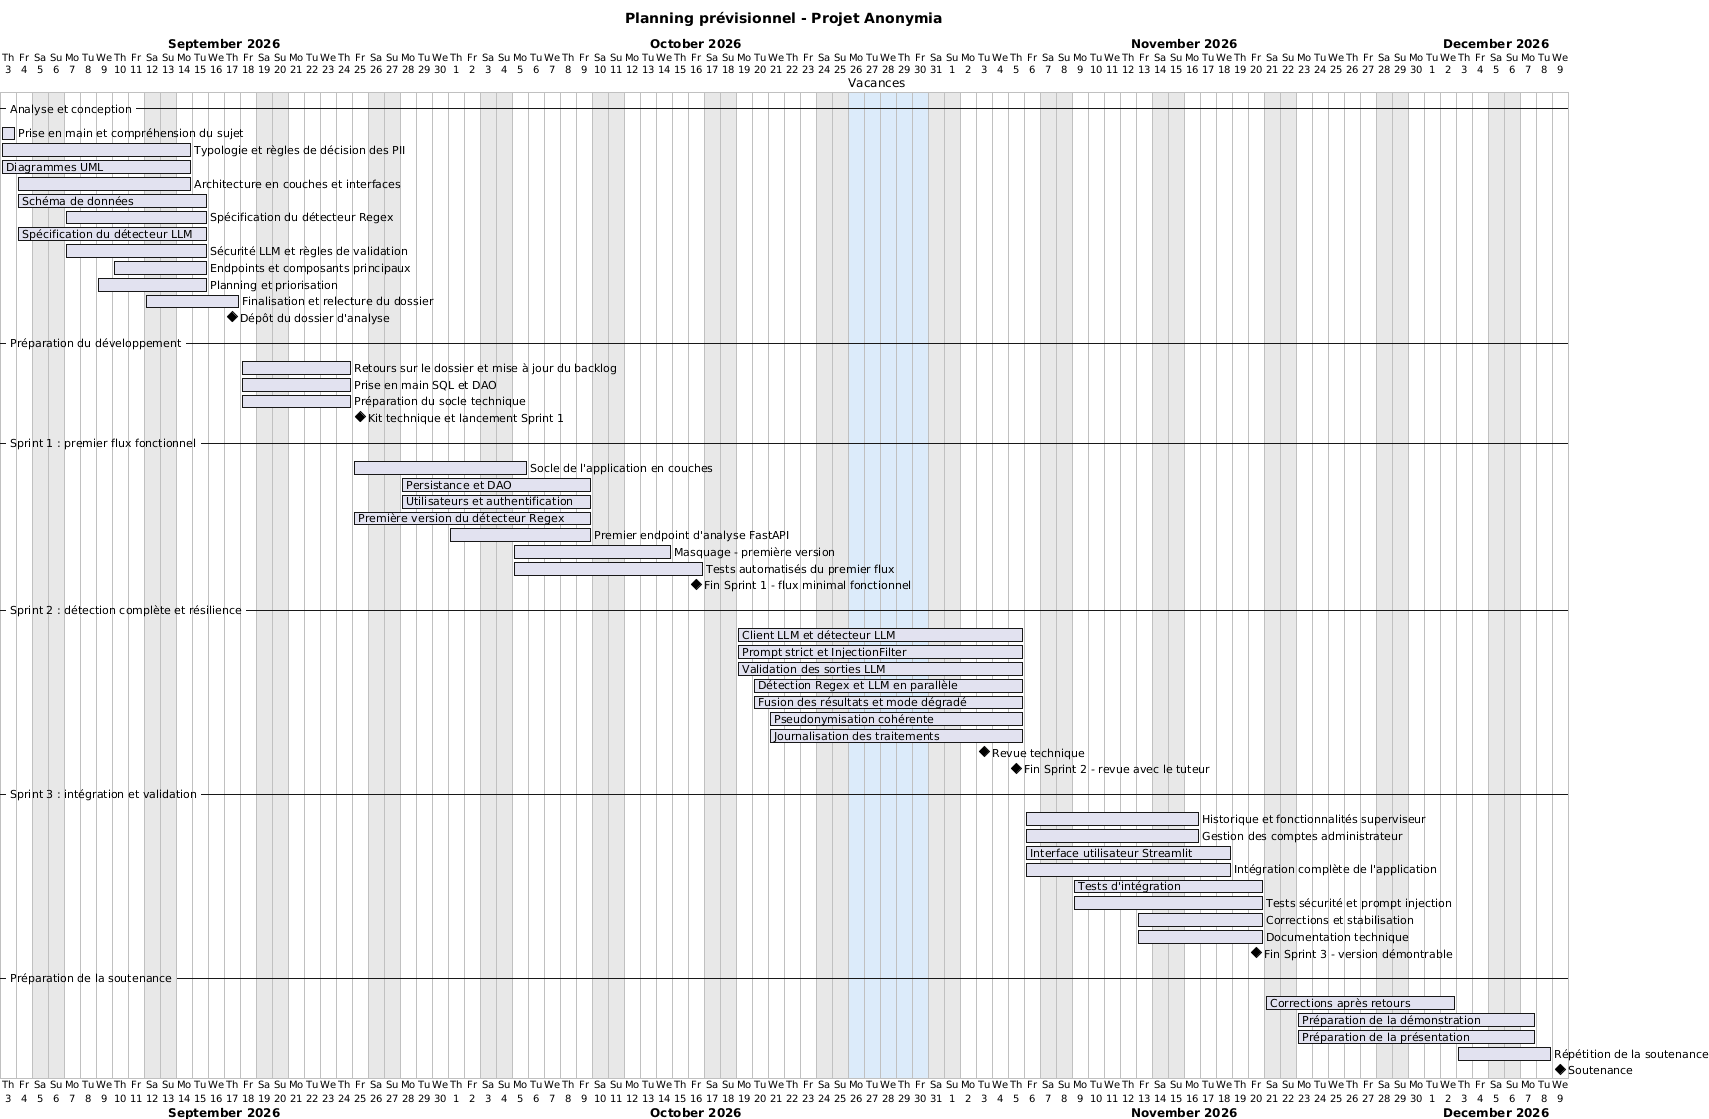
\includegraphics[width=\textwidth]{diagramme_gantt.png}
    \caption{Planning prévisionnel du projet Anonymia}
    \label{fig:gantt}
\end{figure}

Le planning présenté à la figure~\ref{fig:gantt} couvre l'ensemble du projet,
depuis la phase d'analyse jusqu'à la soutenance.

Une première phase est consacrée à l'analyse et à la conception de l'application.
Elle comprend notamment la définition de la typologie des PII, la modélisation UML, la spécification des détecteurs, la définition de l'architecture de l'application ainsi que la préparation du dossier d'analyse, dont le dépôt constitue le premier jalon du projet le 17 septembre.

Après une courte phase de préparation technique, le développement est organisé en plusieurs sprints successifs. Le premier vise à obtenir un premier flux fonctionnel traversant les différentes couches de l'application. Le deuxième approfondit le coeur du système de détection avec l'intégration du LLM, la fusion des résultats des différents détecteurs, la sécurisation des appels au modèle et la gestion du mode dégradé. Le troisième est principalement consacré à l'intégration des fonctionnalités restantes, aux tests et à la stabilisation de l'application.

Nos tests seront réalisés progressivement au cours du développement plutôt que d'être concentrés uniquement à la fin du projet. La dernière phase est consacrée aux corrections éventuelles, à la préparation de la démonstration et à la soutenance prévue le 9 décembre.

Les périodes de week-end et de vacances sont également représentées afin de
prendre en compte la disponibilité réelle de l'équipe. Ce planning reste
prévisionnel et pourra être révisé lors des différentes planifications de sprint en fonction de notre avancement dans la réalisation du projet.

\subsection{Collaboration}
Nous avons décidé de rédiger ce rapport en \textbf{LateX} : pour cela, nous avons décidé d’utiliser \textbf{Overleaf}, une plateforme collaborative classique pour des projets scolaires, que nous avions déjà utilisée en première année. Ce site permet une compilation en temps réel et un aperçu instantané du PDF généré, ce qui permet de vérifier facilement et rapidement le rendu, et ainsi de détecter les éventuelles erreurs de syntaxe et les ajustements de code à faire. De plus, son interface est très intuitive (c’est d’ailleurs la raison pour laquelle ce site nous a été présenté l’année dernière).
L’utilité d’Overleaf est aussi son côté collaboratif, car les documents étant stockés en ligne, ils peuvent être partagés et modifiés à plusieurs simultanément. Cependant, nous avons rapidement découvert qu'il présentait toutefois une limite pour un travail de groupe : sur un compte gratuit, seuls deux membres peuvent éditer le document simultanément. Cette contrainte nous a conduits à utiliser Overleaf uniquement pour une mise en forme finale, et de centraliser tout notre travail préliminaire autre part ; pour cela, nous avons utilisé \textbf{Google Drive} et \textbf{GitHub}.
\newline

\textbf{Google Drive} nous a servis d'espace de travail commun pour tous nos documents en cours d'élaboration : les brouillons des sections, les tableaux récapitulatifs des PII, les versions successives des diagrammes UML... Il nous a permis de collaborer efficacement, car le nombre d'utilisateurs simultanés est illimité. Nous pouvions donc être plusieurs sur un même document en même temps, ce qui était essentiel dans cette phase initiale, où les différents choix de modélisation nous ont demandés plusieurs modifications avant d'être figés. Une fois une section ou un diagramme validé par le groupe, il était reporté dans le LaTeX d'Overleaf.
\newline 

\textbf{GitHub} est une plateforme d'hébergement de dépôts Git dans le cloud, qui permet de stocker du code, donc dans notre cas le code LateX de ce rapport, afin que chacun de nous puisse le modifier, et qu’il soit accessible à ceux qui pouvaient éditer le fichier Overleaf.
Le modèle de Git utilise des commits explicites, ce qui permet de garder une trace des modifications apportées au dossier. De plus, c’est un outil très pratique pour le code, car il détecte les collisions ligne par ligne et autorise à revenir en arrière précisément dans le cas où un changement causerait un problème, ce qui nous est arrivé à plusieurs reprises.
Le dossier GitHub commun contient aussi le suivi hebdomadaire et les fichiers explicitement demandés par le sujet, ce qui permet de juger la qualité de notre travail d'équipe en étudiant la clarté des messages de commit et la régularité de la mise à jour du dossier. 

Les échanges quotidiens de l'équipe passent par un groupe \textbf{WhatsApp}, par exemple pour signaler l'achèvement d'une tâche, demander l'avis sur une direction à prendre, alerter sur un blocage, ou convenir des créneaux de travail commun ou pour demander l'autorisation d'éditer le fichier Overleaf.



\end{document}
